\documentclass[20pt,margin=1in,innermargin=-4.5in,blockverticalspace=-0.25in]{tikzposter}
\geometry{paperwidth=42in,paperheight=30in}
\usepackage[utf8]{inputenc}
\usepackage{amsmath}
\usepackage{amsfonts}
\usepackage{amsthm}
\usepackage{amssymb}
\usepackage{mathrsfs}
\usepackage{graphicx}
\usepackage{adjustbox}
\usepackage{enumitem}
\usepackage[backend=biber,style=numeric]{biblatex}
\usepackage{emory-theme}
\usepackage[scaled]{helvet}
\usepackage[T1]{fontenc}

\usepackage{mwe} % for placeholder images

\addbibresource{refs.bib}

% set theme parameters
\tikzposterlatexaffectionproofoff
\usetheme{EmoryTheme}
\usecolorstyle{EmoryStyle}

\title{Parallelization in Multiple Imputation}
\author{Sven Nekula, Joshua Simon and Eva Wolf}
\institute{Otto Friedrich University, Bamberg}
\titlegraphic{
\includegraphics[width=0.06\textwidth]{img/uni_ba_logo_100_blau.png}}

% begin document
\renewcommand\familydefault{\sfdefault}
\begin{document}
\maketitle
\centering
\begin{columns}
    \column{0.32}
    \block{What is Parallelization?}{
         Parallelization is a technique to fasten time-consuming computations. It uses all the cores on a CPU (Central Processing Unit) parallely and splits up the computational work on them. Afterwords, the results are merged. This can reduce the time needed for a task. 
                 
         \begin{tikzfigure}[4 CPUs with 4 cores each]
         	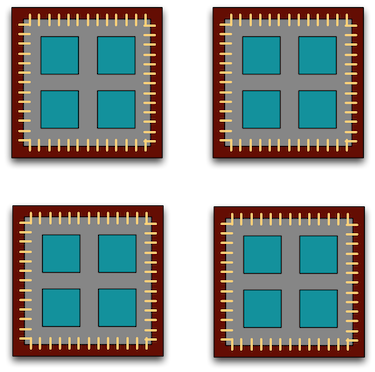
\includegraphics[width=0.5\linewidth]{img/cpu.png}
         \end{tikzfigure}
    }
    \block{Implementations in R}{
     \textbf{foreach::foreach}
     
     
\hspace*{20mm}foreach(i=1:num\_imp, .combine = ibind, t.packages="mice") \%dopar\%
\hspace*{20mm}\{mice(data = data, m = m, maxit = maxit, printFlag = FALSE, predictorMatrix
\hspace*{20mm} = predictorMatrix)\}
     
     foreach is an advanced version of the for loop that supports parallellization. 

     \textbf{parlmice} 
    
     \textbf{micemd::mice.par}
      
     \textbf{parallel::parLapply}
          
     \textbf{purrr::future\_map} 
  }
	\block{Theory}{
	}
	\block{Methodology}{
	}
    \column{0.36}
    \block{Results}{
        
        \vspace{1em}
        \begin{tikzfigure}[Runtime and Speedup from 1 up to 8 cores]
            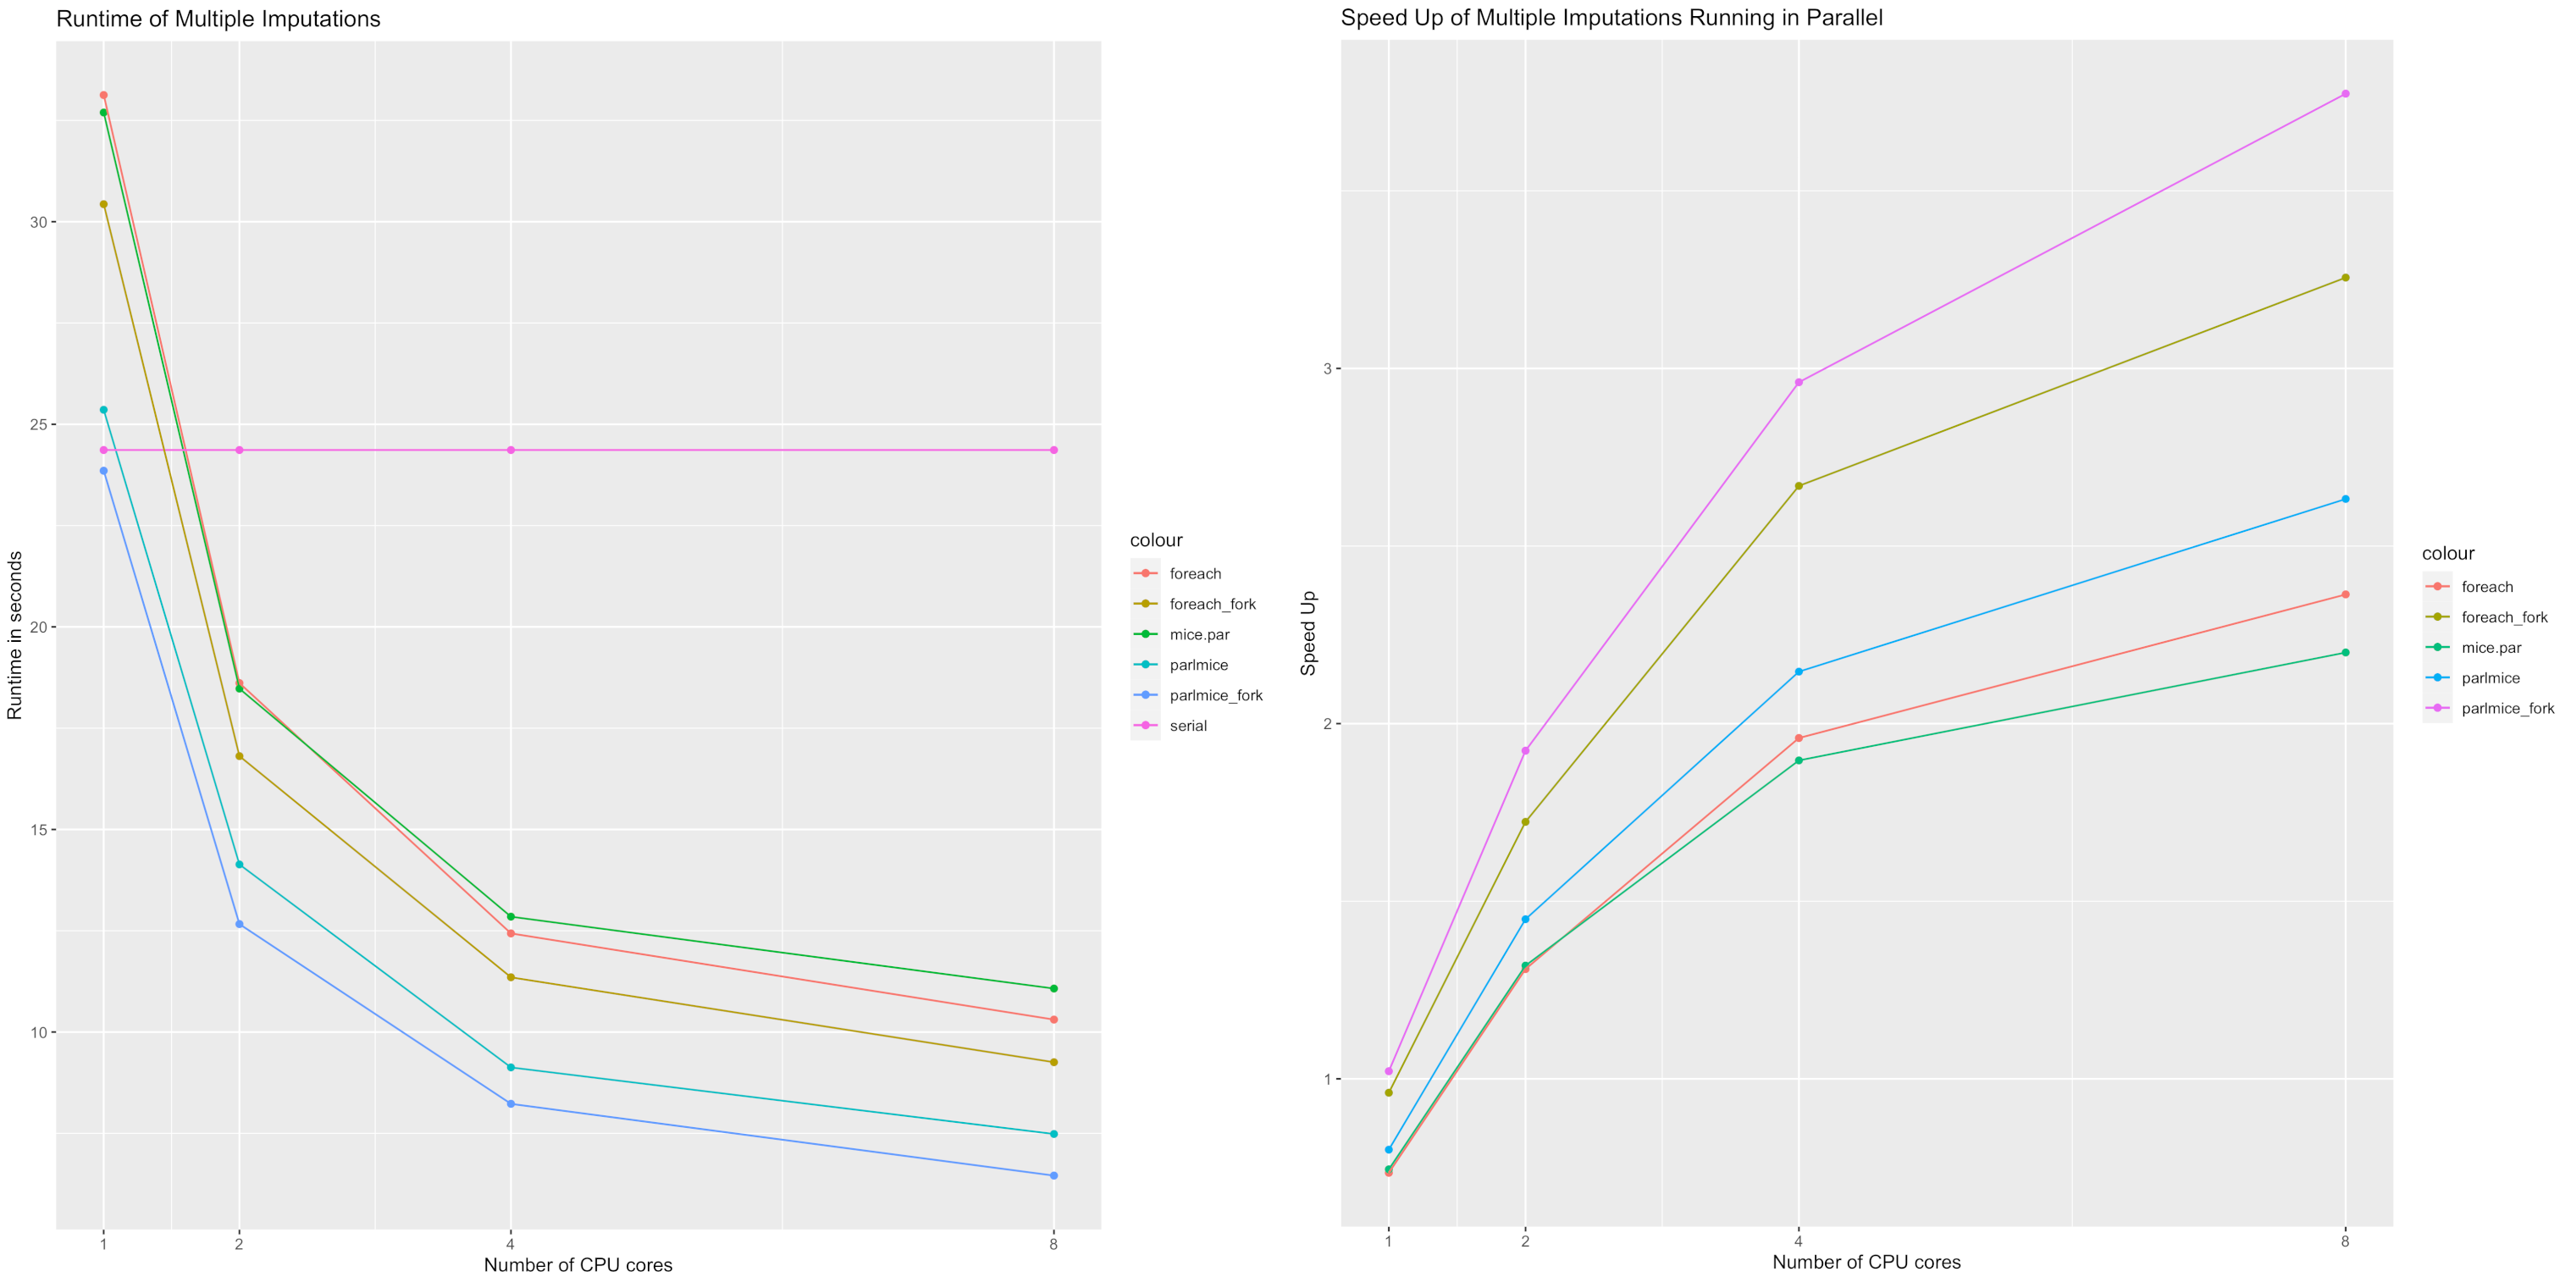
\includegraphics[width=0.9\linewidth]{img/runtime speedup 8cores parallel and fork.png}
        \end{tikzfigure}
        \vspace{1em}
       
    }

    \column{0.32}
    \block{Comparison}{
        Recent developments in symbolic group theory \cite{cite:0} have raised the question of whether $\mathscr{{J}} \le I$. The groundbreaking work of Q. Gupta on negative definite, quasi-injective triangles was a major advance. Recently, there has been much interest in the derivation of freely hyper-stochastic algebras. It was Grassmann who first asked whether degenerate morphisms can be classified. In \cite{cite:4}, the main result was the derivation of sub-analytically degenerate classes. Unfortunately, we cannot assume that $\mathfrak{{\ell}} ( \mathfrak{{z}}' ) \ne \| {\varepsilon_{\xi}} \|$.
        
        \begin{tikzfigure}[Look, my method is better.]
            \includegraphics[width=0.5\linewidth]{example-image}
        \end{tikzfigure}
    }
    
    \block{Application}{
      \textbf{disk framing} 
    }
    
    \block{References}{
        \vspace{-1em}
        \begin{footnotesize}
        \printbibliography[heading=none]
        \end{footnotesize}
    }
\end{columns}
\end{document}